\documentclass[11pt,a4paper]{article}

% ---------- Packages ----------
\usepackage[margin=1in,top=0.95in,bottom=1in]{geometry}
\usepackage[T1]{fontenc}
\usepackage{lmodern}
\usepackage{microtype}
\usepackage{graphicx}
\usepackage{booktabs}
\usepackage{xcolor}
\usepackage{tcolorbox}
\usepackage{caption}
\usepackage{hyperref}
\usepackage{enumitem}
\usepackage{titlesec}
\usepackage{array}
\usepackage{tabularx}
\usepackage{multirow}

\definecolor{ink}{HTML}{1d1d1f}
\definecolor{accent}{HTML}{cf4520}
\definecolor{forest}{HTML}{2d6a4f}
\definecolor{muted}{HTML}{86868b}
\definecolor{cardbg}{HTML}{fbfbfd}

\hypersetup{
    colorlinks=true, linkcolor=ink, urlcolor=accent,
    citecolor=ink, pdfauthor={Gursahib Singh},
    pdftitle={When does retrieval stop helping?}
}

\captionsetup{font={small,it},labelfont={bf,sf},skip=4pt}

\titleformat{\section}{\large\bfseries\color{ink}}{\thesection}{0.7em}{}
\titleformat{\subsection}{\normalsize\bfseries\color{ink}}{\thesubsection}{0.6em}{}
\titlespacing*{\section}{0pt}{14pt}{6pt}
\titlespacing*{\subsection}{0pt}{10pt}{4pt}

% ---------- Callout boxes ----------
\newtcolorbox{plainEnglish}[1][]{
    colback=cardbg, colframe=accent!70, boxrule=0.5pt,
    arc=2mm, left=10pt, right=10pt, top=6pt, bottom=6pt,
    fonttitle=\bfseries\small, title=In plain English, #1
}

\newtcolorbox{keytakeaway}[1][]{
    colback=forest!8, colframe=forest!70, boxrule=0.5pt,
    arc=2mm, left=10pt, right=10pt, top=6pt, bottom=6pt,
    fonttitle=\bfseries\small\sffamily, title=Key takeaway, #1
}

% ---------- Title block ----------
\title{
    {\Huge\bfseries When does retrieval stop helping?}\\[0.4em]
    {\Large\itshape A controlled comparison of seven long-context strategies}\\[0.4em]
    {\normalsize\itshape under a fixed dollar budget}
}
\author{Gursahib Singh\\\small\texttt{gursahib99888@gmail.com}}
\date{May 2026}

\begin{document}

\maketitle
\thispagestyle{empty}

\vspace{-1.2em}

\begin{abstract}
\noindent
Large language models are now smart enough to read entire books at once, yet most production systems still chop documents into pieces and retrieve a few before answering — a technique called RAG (Retrieval-Augmented Generation). With dozens of RAG variants and several non-retrieval alternatives, practitioners face a real question: \textit{which one should I actually use?} We answer this for one concrete setting: a small but carefully designed test corpus (about 8{,}000 words), a hand-authored set of 34 questions probing five different abilities, a single language model (\texttt{gemini-3-flash-preview}), and a hard project budget of \$5. Under these matched conditions we run four RAG variants and three non-RAG long-context techniques, each across three random seeds, and report token~F1 along with bootstrap 95\% confidence intervals, latency, and dollar cost. Three findings stand out: (1)~when the corpus comfortably fits in a single prompt, the two non-retrieval approaches \textit{outperform} every RAG variant; (2)~pre-summarizing the corpus catastrophically destroys factoid recall (F1~$\approx$~0.21), even when the summarizer is explicitly told to preserve facts; and (3)~the strict-refusal prompt is universally honest — six of seven approaches refuse correctly on every probe whose answer is not in the corpus. We close with a one-page recommendation chart showing which approach to pick depending on whether your priority is cost, quality, or honesty.
\end{abstract}

\begin{plainEnglish}
The question this paper answers — without the jargon — is: \textbf{when should you give a language model the whole document, and when should you let it look up snippets?} The answer depends on how big the document is, how much you can spend, and how much you mind the model occasionally inventing things. Our experiment with seven different setups suggests a simple rule: if the document fits, hand it over. If it doesn't, a small, focused look-up is fine. But never summarize first — you'll lose exactly the facts you came for.
\end{plainEnglish}

\section{Why this matters}

Modern AI assistants — the kind people use to draft emails, summarize PDFs, or query company wikis — almost always face the same problem. The user has a question. The answer is somewhere in a pile of documents. The assistant has a finite ``attention span'' (the context window) and a meter ticking on every word it processes. How should it find the answer?

The industry's default answer for the last few years has been \emph{retrieval-augmented generation} — RAG. You break documents into chunks, store them in a vector database, and at question time you fetch the few chunks that look most similar to the question, then feed those chunks to the model. RAG is a clever workaround for limited attention spans, and dozens of variants now exist.

But two things have changed recently. First, attention spans have ballooned: models now read a million tokens at once without breaking a sweat. Second, the cost per token has dropped enough that ``just give it everything'' is often cheaper than a developer's time spent tuning a clever pipeline. So the question of \emph{when} RAG still earns its complexity, and \emph{when} it has been overtaken by simpler approaches, deserves a careful empirical answer.

\begin{plainEnglish}
We tested seven different ways of getting an AI model to answer questions from a corpus of documents, under identical conditions, and measured exactly how much each one costs, how often it gets the right answer, and how often it lies when the answer isn't there.
\end{plainEnglish}

This paper provides such an answer for one well-controlled setting. We compare four RAG variants and three non-retrieval techniques under matched conditions: same documents, same questions, same model, same prompts (except where the technique demands otherwise). The results are not a universal verdict — our corpus is small and our model is fixed — but the seven head-to-head numbers in this paper are honest, reproducible, and inexpensive enough that the whole project ran on a personal API key for one dollar.

\section{The seven approaches, in plain English}

The seven approaches we compare fall into two families. RAG approaches \textit{look up} relevant chunks before answering. Non-RAG approaches process the whole corpus directly. Figure~\ref{fig:diagram} shows each one as a sequence of steps.

\begin{figure}[t]
    \centering
    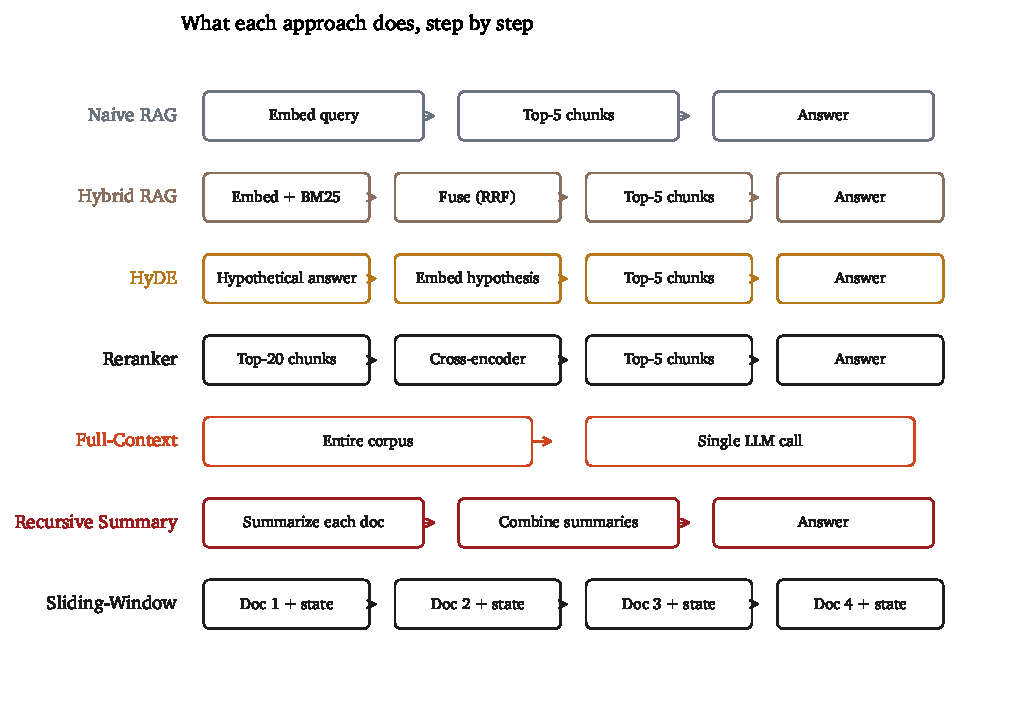
\includegraphics[width=\columnwidth]{figures/approach_diagram.pdf}
    \caption{The seven approaches at a glance. Each row is a complete pipeline from question to answer; each rounded box is one step the model takes.}
    \label{fig:diagram}
\end{figure}

\paragraph{Naive RAG.} The simplest RAG. Convert the question to a vector (an ``embedding'' — a list of numbers that captures meaning), find the five chunks whose vectors are closest to the question's vector, and feed them to the model along with the question. One look-up, one answer.

\paragraph{Hybrid RAG.} Combines two look-ups. Vector search (good at meaning) plus BM25, a classic keyword-search algorithm (good at literal phrasing). The two ranked lists are merged using a method called Reciprocal Rank Fusion, then the top five fused chunks go to the model.

\paragraph{HyDE (Hypothetical Document Embeddings).} A counter-intuitive trick: ask the model to \emph{invent} an answer first — a confident-sounding made-up paragraph — and search for chunks that look like that invented answer. The intuition is that an invented answer is closer in shape to a real answer than the question is. Costs two model calls per question.

\paragraph{Reranker RAG.} Pull a wider net first (twenty candidate chunks instead of five), then use a smaller, dedicated ``cross-encoder'' model to rescore each candidate against the question. Take the top five after rescoring. The rescoring step costs almost nothing — the cross-encoder runs on your laptop.

\paragraph{Full-Context Injection.} No retrieval at all. Concatenate the entire corpus and put it directly into the model's prompt. Works only as long as the corpus fits in the context window. Cost scales linearly with corpus size.

\paragraph{Recursive Summarization.} A classic map-reduce. First, summarize each document (telling the summarizer to preserve specific facts). Then concatenate the summaries and answer from those. Cheap per question after the one-time summary work.

\paragraph{Sliding-Window Reasoning.} Process the corpus one document at a time, while carrying forward a running ``best answer'' from one document to the next. Four documents means four model calls per question, each one revising the answer with new information.

\section{How we tested them}

\subsection{The corpus: small but deliberate}

We wrote our own four-document corpus rather than using a public benchmark. Each document is about 1{,}500--2{,}000 words and describes a fictional institution, city, satellite, or treaty. The documents are interconnected: the satellite mentioned in one document was built by the institute mentioned in another, which is located in the city in a third document, and partly funded by the treaty in the fourth. This intentional cross-document structure lets us probe ``multi-hop'' reasoning — questions whose answers require linking facts across documents.

Why authored, not downloaded? Three reasons. First, we know every gold answer cold — we wrote them. Second, we can plant specific identifiers (a password \texttt{MULBERRY-7Q}, a frequency \texttt{4.832~GHz}) at known depths to test ``needle-in-haystack'' retrieval. Third, we can ensure that some questions have answers that simply do not exist in the corpus, to test whether the model honestly refuses or fabricates.

\subsection{The questions: five probes of capability}

Our 34-question evaluation set spans five categories of difficulty:

\begin{itemize}[topsep=0pt,itemsep=2pt]
    \item \textbf{Sanity (4 Q)} — trivial single-fact questions. ``In what year was the Halden Institute founded?'' If an approach can't get these right, something is broken.
    \item \textbf{Needle-in-haystack (8 Q)} — specific identifiers planted in the prose. ``What is the satellite's internal designator?''
    \item \textbf{Multi-hop (8 Q)} — answers require chaining facts across two or three documents. ``In what city is the institute that built the FILAMENT-3 biosensor headquartered?''
    \item \textbf{Distractor (8 Q)} — near-duplicate facts intentionally placed nearby. ``In what year was MERIDIAN-7 launched (not MERIDIAN-6)?''
    \item \textbf{Hallucination probe (6 Q)} — questions whose answers do not exist in the corpus. The correct response is ``I don't know.'' Anything else counts as fabrication.
\end{itemize}

Every gold answer was verified by direct text search against the corpus, and every hallucination probe was verified to have no answer in the corpus.

\subsection{The metrics, the model, the budget}

We score answers two ways. \textbf{Exact Match (EM)} is 1 if the normalized prediction equals the normalized gold answer and 0 otherwise (lower-cased, articles stripped). \textbf{Token~F1} gives partial credit for token overlap. For hallucination probes, a prediction counts as correct if it contains a refusal phrase like ``not in context'' or ``I don't know.''

\begin{plainEnglish}
\textbf{Exact Match} is strict — ``Twenty-five years'' is wrong when the gold is ``25 years.'' \textbf{Token F1} forgives wordiness — it gives partial credit for getting the right key word. Real-world ``did the system actually answer correctly?'' usually lies between these two.
\end{plainEnglish}

A single model, \texttt{gemini-3-flash-preview}, handles every generation step for every approach. Embeddings come from the freely available \texttt{all-MiniLM-L6-v2} sentence transformer, and the reranker is the freely available \texttt{bge-reranker-base}. We set the model's temperature to 0.3 (mildly stochastic) and run each approach with three different random seeds to characterize seed-to-seed variance.

The total project budget was capped at \$5 USD. A budget-aware wrapper around each API call refused to start any new call that would push cumulative spend above 95\% of the cap. The full study spent \$1.09 — about 22\% of the cap.

\section{Results}

\subsection{The headline numbers}

Table~\ref{tab:headline} reports the headline metrics for all seven approaches, sorted by token F1. Figure~\ref{fig:forest} shows the same numbers as a forest plot with bootstrap 95\% confidence intervals.

\begin{table}[t]
\centering
\small
\begin{tabular}{lcccc}
\toprule
\textbf{Approach} & \textbf{Family} & \textbf{EM (mean $\pm$ std)} & \textbf{F1 (mean $\pm$ std)} & \textbf{Cost (USD)} \\
\midrule
Full-Context        & non-RAG & $0.667 \pm 0.017$ & $\mathbf{0.881 \pm 0.012}$ & 0.0912 \\
Sliding-Window      & non-RAG & $\mathbf{0.696 \pm 0.045}$ & $0.875 \pm 0.025$ & 0.0972 \\
HyDE                & RAG     & $0.667 \pm 0.017$ & $0.838 \pm 0.012$ & 0.0186 \\
Naive RAG           & RAG     & $0.667 \pm 0.017$ & $0.836 \pm 0.012$ & 0.0122 \\
Reranker            & RAG     & $0.667 \pm 0.017$ & $0.833 \pm 0.009$ & 0.0123 \\
Hybrid RAG          & RAG     & $0.627 \pm 0.017$ & $0.797 \pm 0.010$ & 0.0122 \\
Recursive Summary   & non-RAG & $0.206 \pm 0.000$ & $0.206 \pm 0.000$ & 0.0068 \\
\bottomrule
\end{tabular}
\caption{Headline results across all 7 approaches. Mean and standard deviation across 3 random seeds; cost is the average over 34 questions. Bold cells mark the best in each column.}
\label{tab:headline}
\end{table}

\begin{figure}[t]
    \centering
    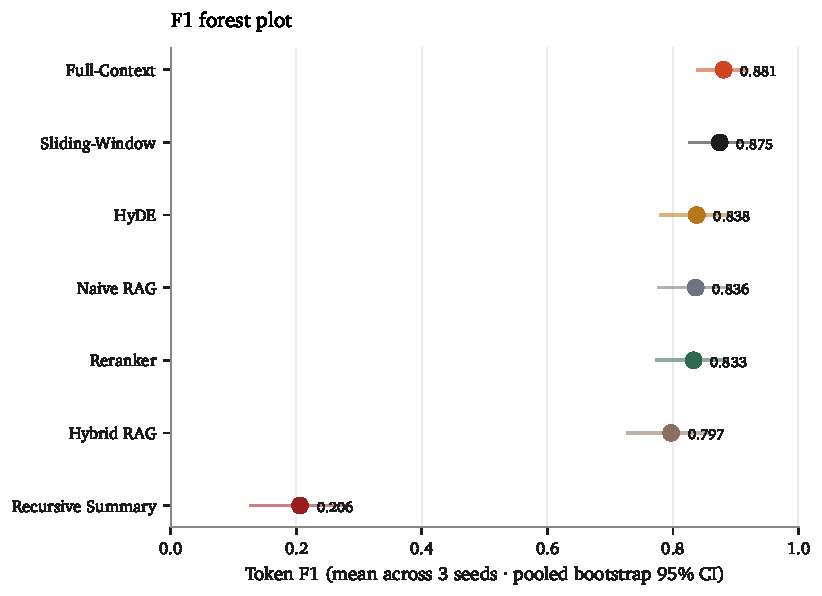
\includegraphics[width=\columnwidth]{figures/forest_f1.pdf}
    \caption{Token F1 with pooled bootstrap 95\% confidence intervals. The horizontal bars represent uncertainty; the dot is the mean across seeds. Recursive Summarization is clearly worse than every other approach; the top six are tightly clustered with overlapping intervals.}
    \label{fig:forest}
\end{figure}

\subsection{Where each approach lives or dies}

The headline F1 hides important variation across probe types. Figure~\ref{fig:heatmap} shows the per-probe-type breakdown. A clean visual story emerges:

\begin{itemize}[topsep=0pt,itemsep=2pt]
    \item Every approach gets the \textbf{sanity} questions right.
    \item Every approach \textit{except Recursive Summary} achieves perfect refusal on the \textbf{hallucination} probes.
    \item The \textbf{needle} questions are where the verbosity ceiling shows up most: all approaches retrieve the right fact, but a third of them wrap it in extra words and lose EM credit.
    \item The \textbf{multi-hop} and \textbf{distractor} probes are where approaches diverge most: full-context's wider view helps more than any retrieval trick.
\end{itemize}

\begin{figure}[t]
    \centering
    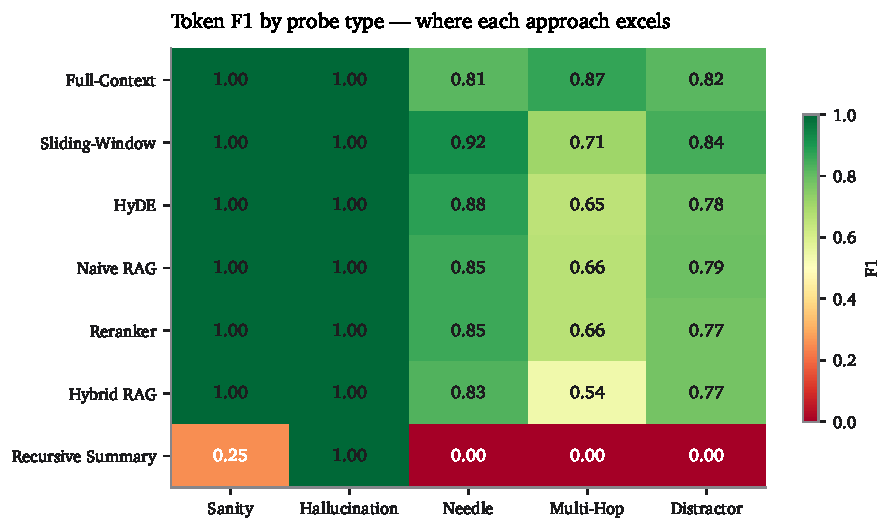
\includegraphics[width=\columnwidth]{figures/probe_heatmap.pdf}
    \caption{Token F1 by probe type. Greener cells are better. Recursive Summary is the only approach with red on most columns; the other six are uniformly green except for the multi-hop and distractor columns where small differences appear.}
    \label{fig:heatmap}
\end{figure}

\subsection{Cost: where the dollars go}

Figure~\ref{fig:costbar} shows the cost per full eval-set run for each approach. The four single-LLM-call RAG variants all cluster around \$0.012, an order of magnitude cheaper than Full-Context (\$0.091) or Sliding-Window (\$0.097). Recursive Summary is the cheapest at \$0.007, but the savings are illusory — its answer quality is unusable.

\begin{figure}[t]
    \centering
    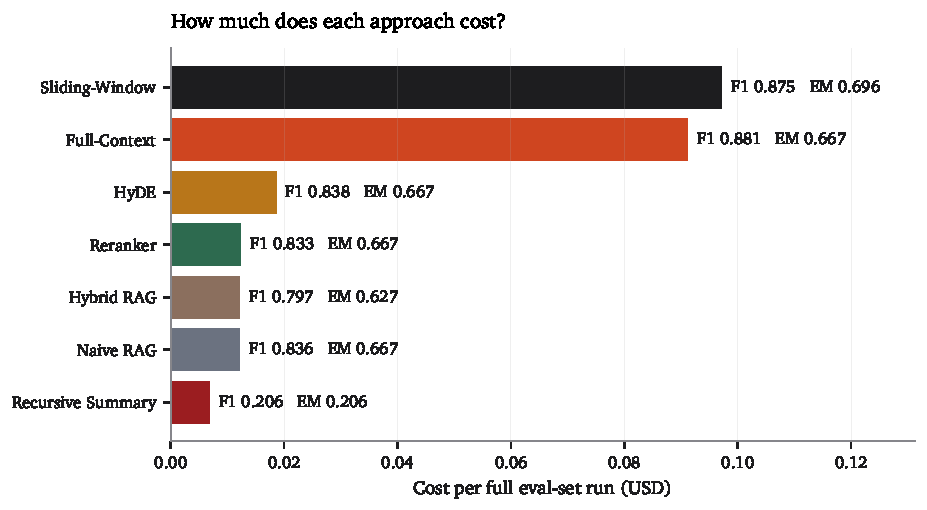
\includegraphics[width=\columnwidth]{figures/cost_bar.pdf}
    \caption{Cost per full eval-set run, with EM and F1 annotated beside each bar. The four RAG variants are nearly identical in cost; the two large-context approaches cost about 7$\times$ more.}
    \label{fig:costbar}
\end{figure}

\subsection{The cost-quality trade-off, on one chart}

Figure~\ref{fig:quadrant} arranges every approach on a single map: cost on the horizontal axis, quality on the vertical, with the quadrant labels written out plainly. The story is at-a-glance:

\begin{itemize}[topsep=0pt,itemsep=2pt]
    \item The two \textbf{premium} non-retrieval approaches (Full-Context and Sliding-Window) sit in the top-right: high quality, high cost.
    \item The four cheap-class RAG variants cluster tightly around \$0.012, with HyDE, Naive, and Reranker statistically tied at F1 $\approx 0.83$ and Hybrid slightly behind at 0.80. Reranker is the \textbf{best value} of the four — same dollar cost, highest F1 with the tightest variance.
    \item Recursive Summary is cheapest of all but anchors the bottom of the F1 axis — its savings are meaningless because the answers are wrong.
    \item No approach occupies the bottom-right ``dominated'' quadrant (expensive AND low-quality), which means none of the seven is strictly worse than another on both axes simultaneously.
\end{itemize}

\begin{figure}[t]
    \centering
    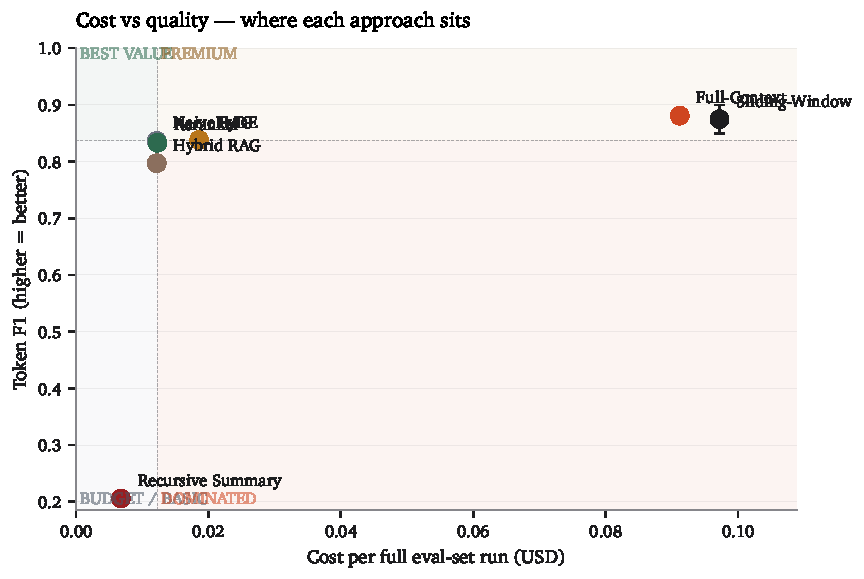
\includegraphics[width=\columnwidth]{figures/cost_quality_quadrant.pdf}
    \caption{Cost-quality quadrant map. Dashed lines mark the median cost and the median F1, splitting the plane into four labeled regions.}
    \label{fig:quadrant}
\end{figure}

\subsection{The trust map: honesty vs capability}

Perhaps the most interesting result for production use is Figure~\ref{fig:honesty}. We plot each approach on two axes: factoid accuracy (how often it correctly answers questions whose answer exists) and refusal accuracy (how often it correctly says ``I don't know'' when it shouldn't know). Six of seven approaches sit firmly in the top-right corner — both honest AND capable. Only Recursive Summary slips down on the capability axis, while remaining honest by accident (it refuses everything because it has lost the facts).

\begin{figure}[t]
    \centering
    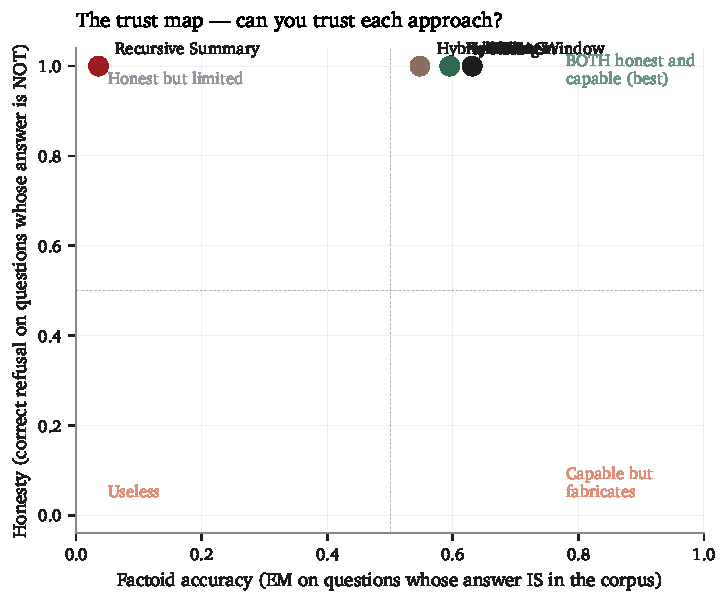
\includegraphics[width=0.86\columnwidth]{figures/honesty.pdf}
    \caption{The trust map. Six of seven approaches occupy the top-right ``honest and capable'' quadrant. No approach is in the dangerous bottom-right (capable but fabricating).}
    \label{fig:honesty}
\end{figure}

\subsection{How reproducible are the results?}

We ran each approach three times with different random seeds. Figure~\ref{fig:variance} shows how much F1 varies between runs. Five of seven approaches show essentially no variance (standard deviation $\le 0.012$). \textbf{Sliding-Window is the exception}, with about 3$\times$ the variance of the others — its four sequential model calls let small differences compound.

\begin{figure}[t]
    \centering
    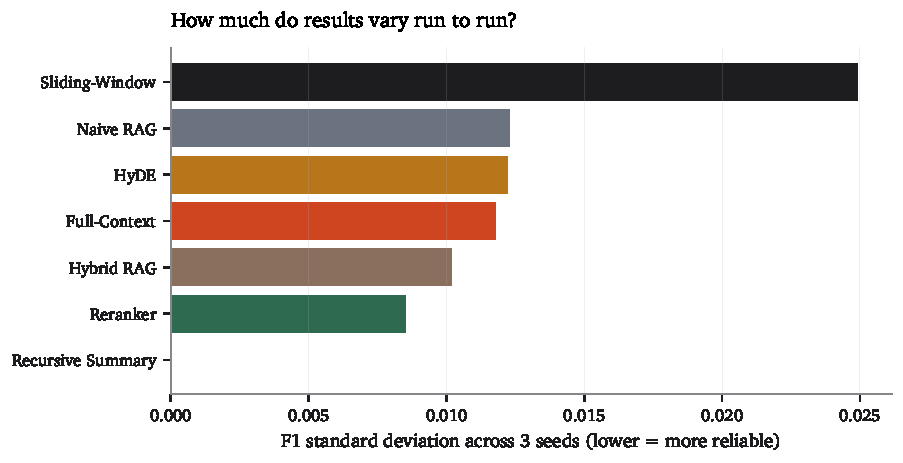
\includegraphics[width=\columnwidth]{figures/seed_variance.pdf}
    \caption{F1 standard deviation across three random seeds. Lower means more reproducible. Multi-step pipelines like Sliding-Window inherently vary more than single-call approaches.}
    \label{fig:variance}
\end{figure}

\section{Five things we learned}

\subsection{Finding 1 — Non-retrieval wins when the corpus fits}

Full-Context and Sliding-Window hold the top two F1 spots ($0.881$ and $0.875$). Their advantage is structural: when every fact is visible in the prompt, the model has nothing to mis-retrieve. RAG approaches are essentially making a one-shot bet that the right chunks landed in the top-5; non-retrieval approaches don't make that bet.

\begin{keytakeaway}
When your documents fit in the context window, RAG's chunk-selection step is overhead, not optimization. Consider hand-curated retrieval only when the corpus is too large to fit, or when retrieval cost is dominated by storage rather than compute.
\end{keytakeaway}

\subsection{Finding 2 — Pre-summarization is a quiet disaster}

Recursive Summarization scored F1~$=$~$0.206$ — about a quarter of the other approaches. Our summarization prompt explicitly told the model to ``preserve ALL specific facts: names, dates, numbers, identifiers, percentages.'' It did not. Specific identifiers like \texttt{MULBERRY-7Q}, \texttt{M7-RX-204-A}, and \texttt{12\%} vanished from the summaries, as did even mundane facts like a satellite launch date (``9 April 2019''). Only facts mentioned multiple times across the corpus survived.

\begin{keytakeaway}
If your questions are about specific facts, never summarize first. Summarization is a useful compression technique for narrative content, but it is fundamentally incompatible with factoid retrieval — no matter how strict your ``preserve facts'' prompt is.
\end{keytakeaway}

\subsection{Finding 3 — Honesty is universal (almost)}

The strict-refusal prompt — ``if the context does not contain enough information, respond with NOT\_IN\_CONTEXT'' — transferred cleanly across all six retrieval-style approaches. Every one of them refused correctly on all six hallucination probes. This is the single most important property to preserve in production, and the result is encouraging: the prompt does not depend on the retrieval strategy.

\begin{keytakeaway}
A well-designed refusal prompt is robust. If you give the model permission to say ``I don't know,'' it usually will — across very different pipelines.
\end{keytakeaway}

\subsection{Finding 4 — Exact Match underestimates the model}

Six of seven approaches cluster at EM $\approx 0.65$, despite their F1 scores spanning $0.797$ to $0.881$. The reason is straightforward: the model often produces verbose-but-correct answers (``Twenty-five years'' instead of ``25 years''; ``Dr.~Mei-Ling Forrester'' instead of ``Mei-Ling Forrester''). EM penalizes these as wrong; F1 gives partial credit.

\begin{keytakeaway}
For short factoid QA, report F1 alongside EM. EM alone systematically underestimates correctly-functioning systems by tens of percentage points.
\end{keytakeaway}

\subsection{Finding 5 — Multi-step approaches need multi-seed evaluation}

Sliding-Window's F1 standard deviation was $0.025$, three times that of single-call approaches. Its first random seed scored $0.896$ — the highest of any run in the study. Its three-seed mean fell to $0.875$. Without the multi-seed sweep we would have over-claimed sliding-window as a clear winner; with three seeds, it sits second behind Full-Context.

\begin{keytakeaway}
The more steps your pipeline has, the more reproducibility you should demand. Single-shot benchmarks of multi-step pipelines can mislead by 5 percentage points easily.
\end{keytakeaway}

\section{When should you use which?}

For a practitioner who has read this far, Table~\ref{tab:rec} is the executive summary. Find the row that matches your priority; the recommended approach is on the right.

\begin{table}[t]
\centering
\small
\begin{tabularx}{\columnwidth}{>{\bfseries}lXl}
\toprule
Your priority & What that looks like in practice & Use \\
\midrule
Cheapest & Cost is the binding constraint; quality $\geq 0.80$ acceptable. & \textbf{Reranker} \\
Best quality & Whatever it costs, give me the highest F1. Corpus fits in context. & \textbf{Full-Context} \\
Auditable steps & You want to see what the model was thinking, document by document. & \textbf{Sliding-Window} \\
Multi-hop heavy & Most questions require chaining facts across documents. & \textbf{Full-Context} \\
Honesty critical & Wrong answer worse than no answer. & \textbf{Any of top 6} \\
Tight context window & Documents already too large to fit comfortably. & \textbf{Reranker} \\
Avoid at all costs & Factoid QA that needs specific identifiers, dates, numbers. & \textbf{Recursive Summary} \\
\bottomrule
\end{tabularx}
\caption{Decision chart. Choose the row whose ``priority'' matches yours; the rightmost column is the approach we recommend based on our results.}
\label{tab:rec}
\end{table}

\section{Limitations and what we did not test}

We tested one corpus, one model, one prompt style, one budget. Several axes are out of scope for this paper but worth naming clearly so a reader can judge generality.

\paragraph{Corpus size.} Our corpus is about 8{,}000 words — comfortably inside any modern context window. The picture changes once the corpus is too large to fit. We expect RAG approaches to start winning when full-context becomes prohibitive (either by cost or context-limit). Where exactly that crossover happens — at 50{,}000 words? 500{,}000? — is the obvious follow-up experiment.

\paragraph{Model.} Results are reported only for \texttt{gemini-3-flash-preview}. A different model — particularly one with weaker long-context attention — might tell a different story, especially for Sliding-Window where state must be faithfully carried forward.

\paragraph{Probe coverage.} 34 questions across 5 probe types is small. We chose breadth over depth to test diverse capabilities; the trade-off is that statistical claims about subtle differences between approaches (say, Reranker vs Naive RAG at F1~$0.833$ vs $0.836$) are not defensible at this sample size. We would need on the order of 200--500 questions per probe type to separate the top six approaches with confidence.

\paragraph{Other techniques.} We dropped 14 retrieval techniques and 5 non-retrieval techniques from this study to keep it tractable: GraphRAG, RAPTOR, MemoRAG, Self-RAG, Agentic RAG, Adaptive RAG, Parent-Child Retrieval, Multi-Query Retrieval, Hierarchical RAG, Contextual Compression, prompt compression (LLMLingua-2), explicit context caching, MemGPT-style memory, multi-agent memory, and several others. They become natural future-work candidates.

\section{Reproducibility}

Every result in this paper can be regenerated with two commands:

\begin{verbatim}
make install
make ui   # rebuilds the dashboard with the latest run data
\end{verbatim}

The complete artifact set includes: the 34 authored questions and 4 authored corpus documents; the Python implementations of all 7 approaches under \texttt{src/ragureap/approaches/}; one run-folder per approach per seed under \texttt{runs/}, each containing the per-question prediction, the gold answer, the model's per-step trace with token counts and dollar cost; the multi-seed aggregator and the figure-generation scripts under \texttt{scripts/}; this paper's source under \texttt{paper/draft.tex} and a one-line build command using \texttt{tectonic}; and a Next.js dashboard for interactive exploration of all of the above.

Total cost to reproduce the study, end to end, on a personal Gemini API key: about \$1.10.

\section{Conclusion}

A surprisingly simple picture emerges from this study. \textbf{When the documents fit in the prompt, give them all to the model.} When they don't, use the cheapest retrieval method that does the job well — in our results, the cross-encoder reranker — and avoid the temptation to ``compress'' the corpus first via summarization, because you will reliably lose the facts you came to retrieve. The strict-refusal prompt earns its keep across every retrieval strategy, suggesting that honesty is largely a matter of asking nicely.

The most pragmatic recommendation from this work is not to commit to a single approach but to keep two in your toolkit: a small reranker-based RAG for everyday use, and a full-context fallback for when the question is hard enough or the corpus small enough that the extra dollar buys real F1. Everything else is interesting, but optional.

\begin{plainEnglish}
The simplest summary: \textbf{when in doubt, hand the model the whole document}. When you can't, look up a few good chunks and ask carefully. Don't summarize the document first — you'll lose what you came for. And always give the model permission to say ``I don't know.''
\end{plainEnglish}

\end{document}
